\documentclass[a4paper]{article}

\usepackage{hyperref}
\usepackage{inputenc}
\usepackage{amsmath}
\usepackage{graphicx}
\usepackage{subcaption}

\usepackage{biblatex}
\addbibresource{bibfile.bib}

\title{CSE 300 Online 2}
\author{Your ID}
\date{July 5, 2019}

\begin{document}
\maketitle
\section{Graphics}
Emacs, Nano, or Vim:  Choose your Terminal-Based Text Editor Wisely.
Nano is the built-in basic text editor for many popular distros. 
 Its usually alreadycontained  in  the  distro, 
  doesnt  take  any  learning  or  getting  used  to,
   and  allits commands and prompts are displayed at the bottom. 
  Nano is the built-inbasic text editor for many popular distros.  Its usually already contained in thedistro, doesnt take any learning or getting used to, and all its commands andprompts are displayed at the bottom.  Vi or one of its variants typically comeswith  your  distro-of-choice.   Its  considered  a  modal  editor,  which  means  thereare different modes for navigating files and editing text.  Because you navigateVi most efficiently through the use of keyboard commands and shortcuts, Vi isbetter experienced than explained.
\begin{figure}[h!]
	\centering
	\begin{subfigure}{0.3\linewidth}
		
\includegraphics[scale=0.1,width = \linewidth]{emacslogo.png}
		\caption{Emacs}
	\end{subfigure}
	\begin{subfigure}{0.3\linewidth}
		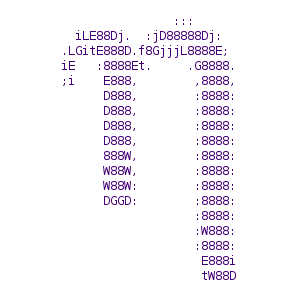
\includegraphics[scale=0.4,width = \linewidth]{nanologo.png}
		\caption{Nano}
	\end{subfigure}
	\begin{subfigure}{0.3\linewidth}
		
\includegraphics[scale=0.1,width = \linewidth]{vimlogo.png}
		\caption{Vim}
	\end{subfigure}
	
	\caption{Terminal-based text-editors}
	\label{ides}
\end{figure}
\section{Equations}
In algebra,
a quadratic equation is any equation having the form
$ax^2+bx+c= 0$ where $x$ represents an unknown
, and $a$,$b$, and $c$ represent known numbers,
 with  $a \neq 0$.   It  can  easily  be  seen, 
  by  polynomial  expansion,  that  the  following 
  equation is equivalent to the quadratic equation:
\begin{equation*}
	\left(x + \frac{b}{2a}\right)^2 = \frac{b^2 - 4ac}{4a^2}
\end{equation*}
Taking the square root of both sides, and isolating $x$,gives:
\begin{equation}
	x = \frac{-b+\sqrt{b^2-4ac}}{2a}
\end{equation}
\subsection*{Some Equations:}
$$ f_1(t) = \int^5_3 \sin(x) dx $$
$$ 
	F(x) = A_0 + \sum_{n=1}^{N}\left[A_n \cos \left(\frac{2\pi n x }{P} \right) + B_n \sin \left( \frac{2\pi n x }{P} \right) \right]
$$
$$
	\lim_{x\to a} \frac{f(x) -f(a)}{x-a}
$$
$$
	\binom{a}{b+c} \binom{\frac{n^2-1}{2}}{n+1}
$$
$$
	h \leq \sqrt{\frac{(s-a)(s-b)(s-c)}{s}}
$$
$$
	6CO_2 + 6H_2O \to C_6H_12O_6 + 6O_2
$$
\begin{equation}
	\left[
	\begin{matrix}
		a_1 & a_2 & a_3 \\
		b_1 & b_2 & b_3 \\
		c_1 & c_2 & c_3 
	\end{matrix}
	\right]
\end{equation}

\section{Bibliography}
The recent success of neural networks has boosted research 
on pattern recog-nition and data mining.
  Many machine learning tasks such as object detection
  in ``You Only Look Once” \cite{redmon2016you} ,
   machine translation \Cite{luong2015effective},
and speech recognition \Cite{hinton2012deep},
 which once heavily relied on handcrafted feature 
 engineering to extract in-formative feature sets,
  has recently been revolutionized by various 
  end-to-enddeep learning paradigms,
    i.e.,  convolutional neural networks 
	(CNNs) \Cite{lecun1995convolutional},
longshortterm memory (LSTM) \Cite{hochreiter1997long},
 and autoencoders.
\newpage
\printbibliography
\end{document}
